\section{University of Hawai'i Cluster}

\subsection{{\craycs}}
\begin{frame}
\frametitle{{\craycs} -- History}
\begin{itemize}
\item[] 2014
  \begin{itemize}
  \item Jul. -- University of {\hawaii} (UH) selects Cray's proposal
  \item Oct. -- Delivered 184 nodes, 3,800 cores
  \item Dec. -- Passed testing and accepted
  \end{itemize}

\item[] 2015
  \begin{itemize}
  \item Jan. -- Early adopter testing started (8 users)
  \item Apr. -- Opened for general use
  \end{itemize}
\item[] 2016
  \begin{itemize}
  \item Mar. -- 92 nodes added, 5,876 cores total
  \end{itemize}
\item[] 2017
  \begin{itemize}
  \item Jan. -- 5 nodes added, 5,992 cores total
  \item Jan. -- 370$+$ users have been granted access to the cluster
  \end{itemize}
\end{itemize}
\end{frame}


\subsubsection{Hardware}
\begin{frame}
	\frametitle{{\craycs} -- Compute Nodes}
	\begin{itemize}
        \item All nodes are diskless with some RAM used for the Operating System
	\item 178 Standard nodes {\tiny(\emph{community})}
	  \begin{itemize}
            {\footnotesize
	    \item Two 10 core {\intel} Ivy-Bridge processors (\emph{20 cores total})
	    \item 128GB of physical RAM with $\approx118$GB of useable RAM
            }
	  \end{itemize}          
	\item 6 Large memory nodes {\tiny(\emph{community})}
	  \begin{itemize}
            {\footnotesize
	    \item Four 10 core {\intel}  Ivy-Bridge processors (\emph{40 cores total})
	    \item 1TB of physical RAM with $\approx1000$GB of useable RAM
            }
	  \end{itemize}			
        \item 1 GPU node {\tiny(\emph{community})}
          \begin{itemize}
            {\footnotesize
	    \item Two 10 core {\intel} Haswell processors (\emph{20 cores total})
	    \item 128GB of physical RAM with $\approx118$GB of useable RAM
            \item 2 Nvidia Tesla K40 GPUs
            }
	  \end{itemize}
        \item 96 Owner nodes
          \begin{itemize}
            {\footnotesize
            \item 33 nodes have two 10 core {\intel} Haswell processors with 256 GB of RAM
            \item 62 nodes have two 12 core {\intel} Haswell processors with 128 GB of RAM
            \item 1 GPU node
            }
          \end{itemize}
	\item CentOS Linux
	\end{itemize}
\end{frame}


\begin{frame}
	\frametitle{{\craycs} -- Storage}
	Two storage options are currently available on the {\craycs}
	\begin{enumerate}
		\item {\lustre}
                  \begin{itemize}
                  \item High performance parallel filesystem 
                  \item Available on all the cluster nodes
                    \item Freely available to all users
                  \end{itemize}
		\item ValueStorage
                  \begin{itemize}
                  \item Network attached scale out storage
                  \item Only available from the login nodes
                  \item Available as a for fee service
                  \end{itemize}
	\end{enumerate}
\end{frame}


\begin{frame}
	\frametitle{{\craycs} -- Storage $\rightarrow$ {\lustre}}
	\begin{itemize}
		\item The {\craycs} has $\approx582$TB of storage space

		\item Primarily used as scratch space for jobs (Input and Output)
		\item User do not have a usage quota (soft or hard)
		\item Certain directories are subject to a 90 day purge policy
		\item \textbf{Data is not backed up!  Users are responsible for their own data}
                \item {\lustre} utilizes RAID 6 arrays, and is fairly robust but \ldots~\\RAID is not a backup
	\end{itemize}
\end{frame}


\begin{frame}
	\frametitle{{\craycs} -- Storage $\rightarrow$ ValueStorage}
        ~\\
	\begin{itemize}
		\item $500$TB of scale out storage
		\item Purchased annually in 0.5TB increments 
	\end{itemize}
	\btVFill

	\begin{center}
	\textbf{ValueStorage Pricing}~\\ 
		\resizebox{0.50\textwidth}{!}{%
		\begin{tabular}{l r }
			\toprule
			\textbf{Product} & \textbf{Annual Cost}~~ \\
	                \midrule
			\midrule
			0.5TB & \$65.00\\
                        0.5TB + Replication  & \$130.00 \\
			\bottomrule
		\end{tabular}
		}
		~\\ \href{http://www.hawaii.edu/its/value-storage-pricing/}{More Information}
		~\\	{\footnotesize \emph{All prices are subject to change}}
	\end{center}
\end{frame}


\begin{frame}
	\frametitle{{\craycs} -- Network}
	\begin{itemize}
		\item 40Gb Infiniband inter-connects (QDR)
		\begin{itemize}
			\item High speed inter-connect between~\\compute nodes, {\lustre} storage and Login nodes
                        \item low latency ($\approx1.3\mu$s)
			\item Utilizes the \emph{fat tree network topology}
			\item[] 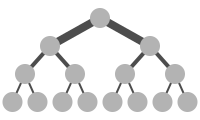
\includegraphics[width=0.20\textwidth]{images/Fat_tree_network} \\[-1ex] {\fontsize{3}{4} \selectfont Source: \url{https://en.wikipedia.org/wiki/Fat_tree} } 		
		\end{itemize}
		\item 10Gb login node internet connectivity
		\begin{itemize}
			\item Speed test from UH to CERN clocked transfer speeds up to 2$+$ Gb/s
		\end{itemize}	
	\end{itemize}
\end{frame}

\subsubsection{Layout}
\begin{frame}
	\frametitle{{\craycs} -- Layout}
	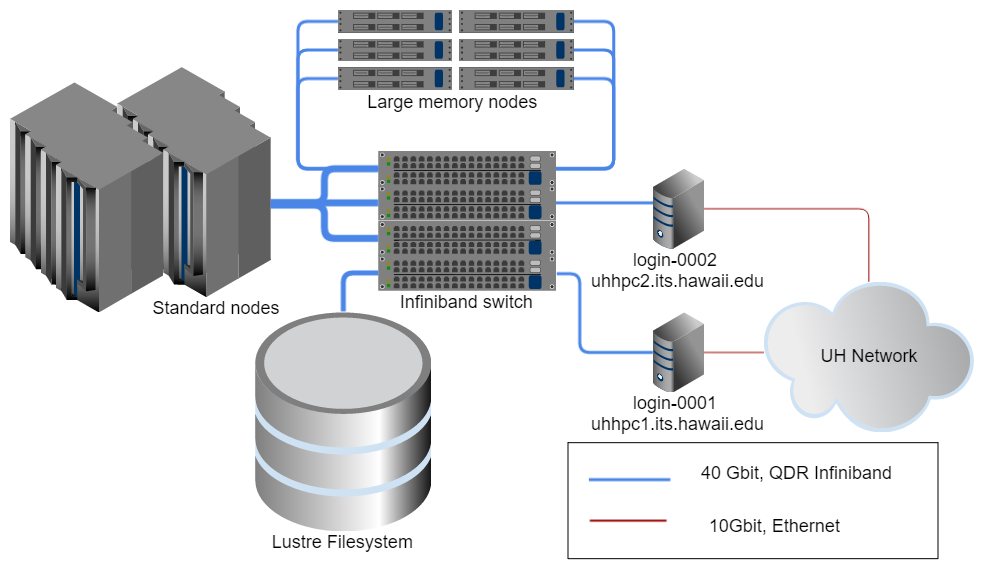
\includegraphics[width=1\textwidth]{images/layout}
\end{frame}

